\documentclass[]{article}
\usepackage[margin=0.9in]{geometry}

\usepackage{enumitem}
\usepackage{graphicx}
\usepackage{hyperref}
\usepackage{float}
\usepackage{fancyvrb,newverbs,xcolor}

\usepackage{listings}
\lstset{
	language=bash,
	basicstyle=\ttfamily
}

\providecommand{\tightlist}{%
	\setlength{\itemsep}{0pt}\setlength{\parskip}{0pt}}


% Back tick style from gfm
\definecolor{Light}{gray}{.90}

\let\oldtexttt\texttt
\renewcommand{\texttt}[1]{
	\colorbox{Light}{\oldtexttt{#1}}
}

\graphicspath{{images/user-manual/}{images/logo/}}

\hypersetup{
	colorlinks=true,
	linkcolor=blue,
	filecolor=magenta,
	urlcolor=cyan,
}

%opening
\title{User Manual for Docks\\
\large{docks-ui 0.0.2}}

\author{TripleParity}
\date{}

\begin{document}

\maketitle

\begin{figure}[H]
	
\includegraphics[scale=0.7]{docks_round_512.png}
	\centering
\end{figure}

\tableofcontents

\section{System Overview}
Docks is a system to manage a Docker Swarm using a Web User Interface. It provides a visual representation of a Docker Swarm, allowing users to manage the Swarm without using the Command Line Interface.

Docks is useful if you want to see a quick overview of the Swarm and all the running containers. Containers can be started and stopped with the click of a button.

System Administrators will be able to effectively manage their Swarm and scale services as required. Docks also appeals to users wishing to manage their services remotely from a web browser.

\section{System Configuration}
Docks consists of two subsystems; the Docks API server and the Docks UI.

The Docks API server has to be on a Manager Node in the Docker Swarm to be able to manage other nodes. The Docks UI also has to be served from the same Domain Name as the Docks API, in most cases it will also by deployed on the Manager Node.

\begin{figure}[h!]
	\centering
	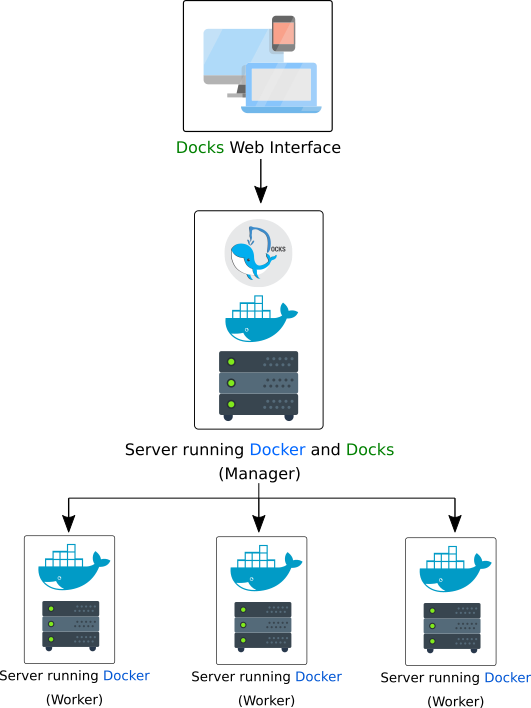
\includegraphics[scale=0.8]{deployment_diagram.png}
	\caption{Docks Deployment Diagram}
\end{figure}

\pagebreak

\section{Installation}
% This section was generated by Pandoc from the README.md
% $ sudo dnf install pandoc
% $ pandoc -s README.md -o README.tex
% Copy Getting Started section to this document
% Fix links or anything that was not successfully converted to latex

\begin{enumerate}
	\def\labelenumi{\arabic{enumi}.}
	\tightlist
	\item
	  Install \href{https://docs.docker.com/install/}{Docker} 17.06.2-ce or higher
	\item
	  Install \href{https://docs.docker.com/compose/install/}{Docker Compose}
	\item
	  Create a Swarm using \texttt{sudo\ docker\ swarm\ init}
	\item
	  Clone \texttt{https://github.com/TripleParity/docks.git}
	\item
	  Run \texttt{sudo\ docker-compose\ pull} to download the required
	  images
	\item
	  Run
	  \texttt{sudo\ docker\ stack\ deploy\ -c\ docker-compose.yml\ docks} to
	  deploy Docks
	\item
	  Run
	  \texttt{sudo\ docker\ stack\ deploy\ -c\ docker-compose-nginx.yml\ demo}
	  to deploy a sample application
	\item
	  Browse to \url{http://127.0.0.1:4200} to view the Docks web interface
	\item
	  To remove Docks from the system run the following commands:
	
	  \begin{itemize}
	  \tightlist
	  \item
		\texttt{sudo\ docker\ stack\ rm\ docks}
	  \item
		\texttt{sudo\ docker\ stack\ rm\ demo}
	  \end{itemize}
	\end{enumerate}


\section{Getting Started}
The web interface will be available at \url{http://127.0.0.1:4200} after following the Installation instructions.
All required setup should be automatically done when starting the Docks stack.

The home screen should display when visiting \url{http://127.0.0.1:4200}

\begin{figure}[H]
	\centering
	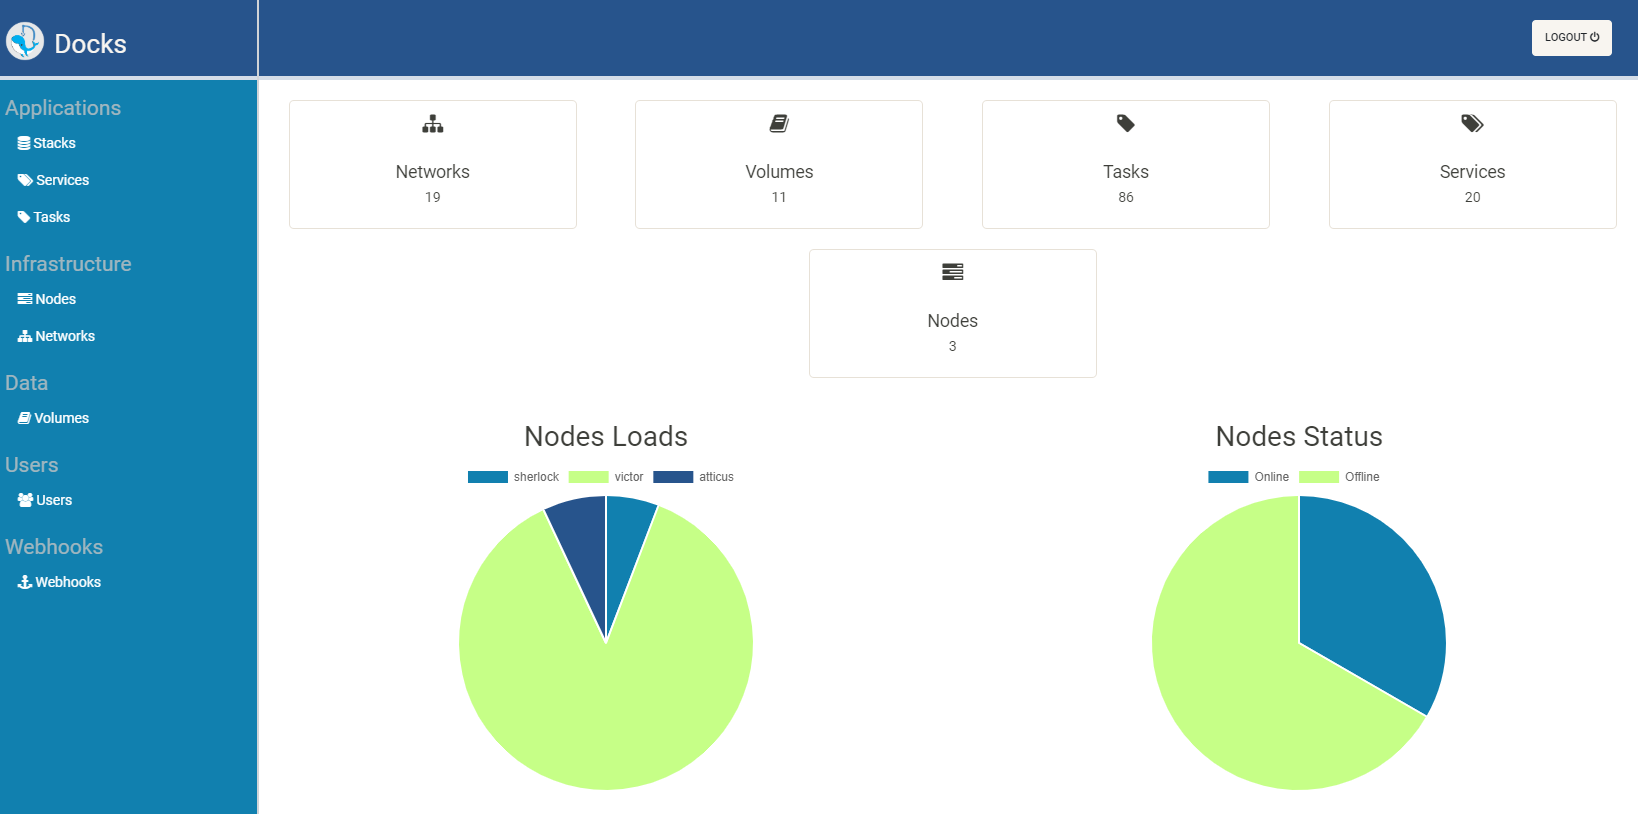
\includegraphics[scale=0.4]{home.png}
	\caption{Home Screen}
\end{figure}

\section{Using the System}

\subsection{Views}
All information can be viewed in two ways, as a list or as cards. The list view is more compact but provides less
information initially. This is useful for seeing a summary of all running resources. Card view provides more detail
without extra information and therefore fewer resources can be seen at a time. Card view is useful if you
need to see more detailed information at a quick glance.

\subsection{Tasks}
Tasks are the containers associated with a running service. On the task list view you can see the task ID and it's state. Upon clicking on a task in the list it will expand to also show the node ID the task is running on, the image the task was created from, the date created and the date update.

\begin{figure}[H]
	\centering
	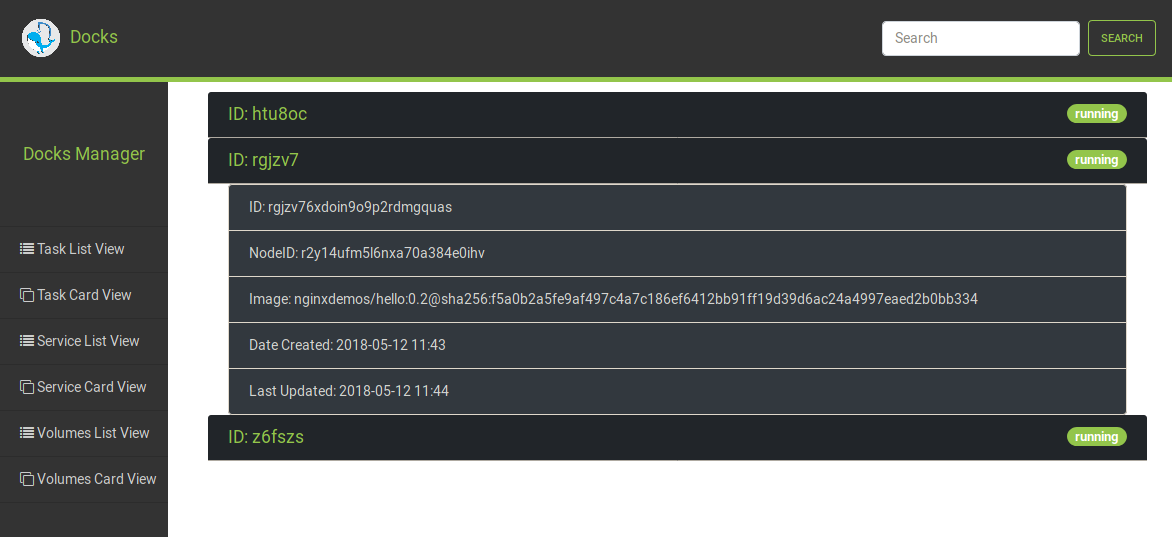
\includegraphics[scale=0.4]{task_list.png}
	\caption{Task list view, with one task expanded}
\end{figure}

The card view displays the following information:
\begin{itemize}
	\tightlist
	\item ID of the task
	\item State of the task. Indicated by the circle and card outline colour. Green means the task is running, red indicating it has stopped
	\item Node ID the task is running on
	\item Last Updated
\end{itemize}

\begin{figure}[H]
	\centering
	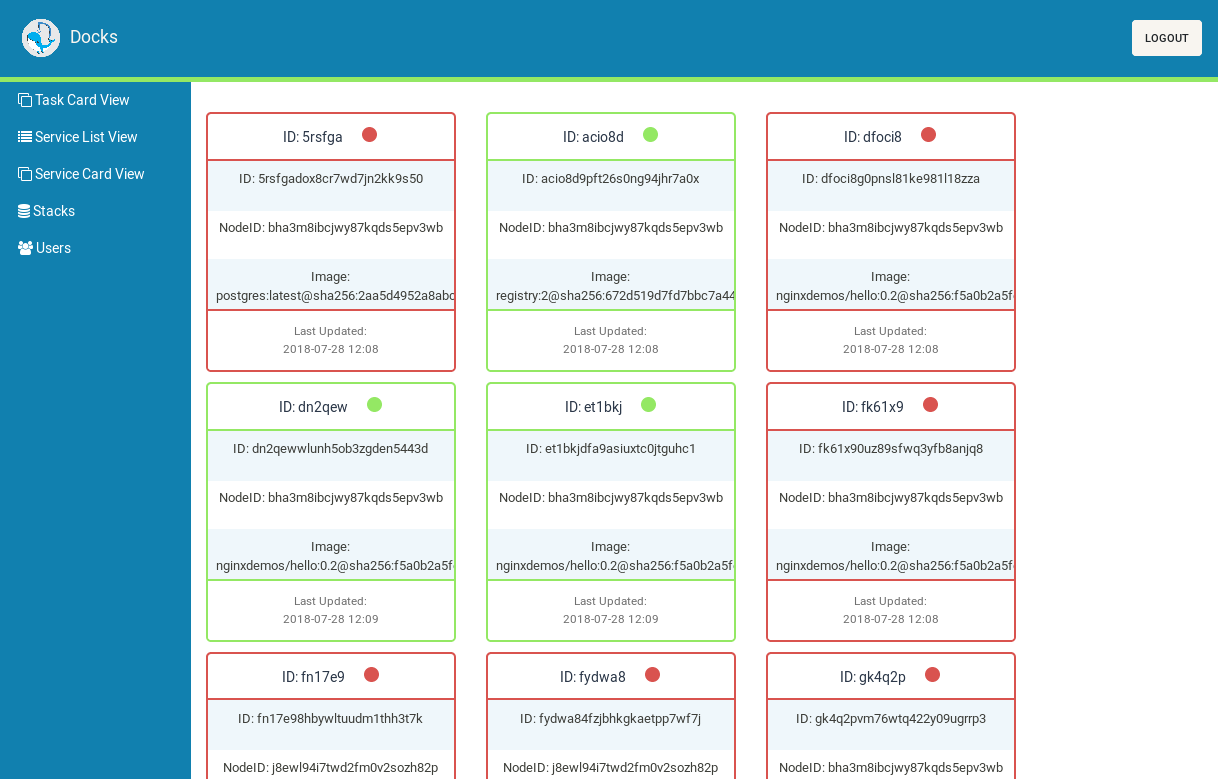
\includegraphics[scale=0.4]{task_card_view.png}
	\caption{Task card view}
\end{figure}

Cards can be clicked on to bring up a modal dialog to display the log for that service.

\begin{figure}[H]
	\centering
	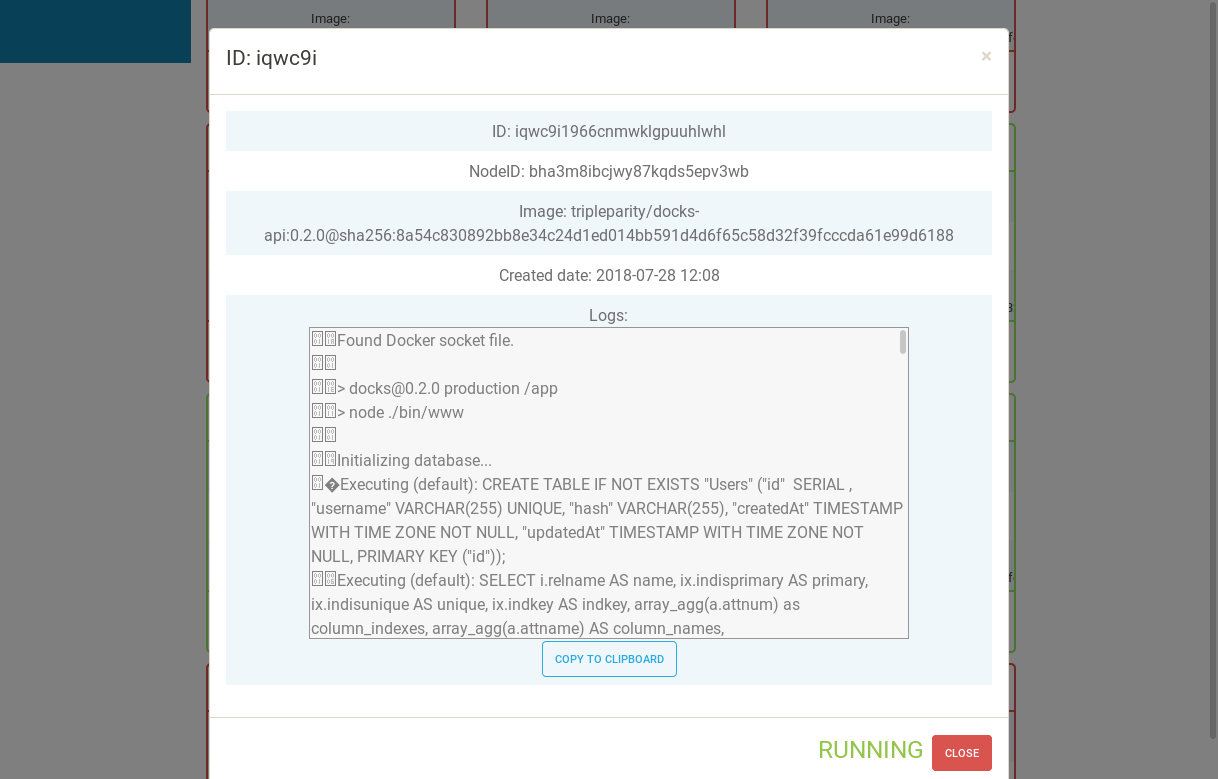
\includegraphics[scale=0.4]{task_card_modal.png}
	\caption{Task modal after clicking on card. Displays task log}
\end{figure}

\subsection{Services}

The services list view displays a list of services, which can be clicked on for an expanded view:
\begin{itemize}
	\tightlist
	\item Image the service is created from
	\item The mode of the service. \texttt{vip} - Virtual IP, the service is assigned an IP address and will distribute the requests to the replicated tasks.
	\item The number of replicas of the service. Each replica represents a task in the swarm.
	\item Date crated
	\item Last updated
\end{itemize}

\begin{figure}[H]
	\centering
	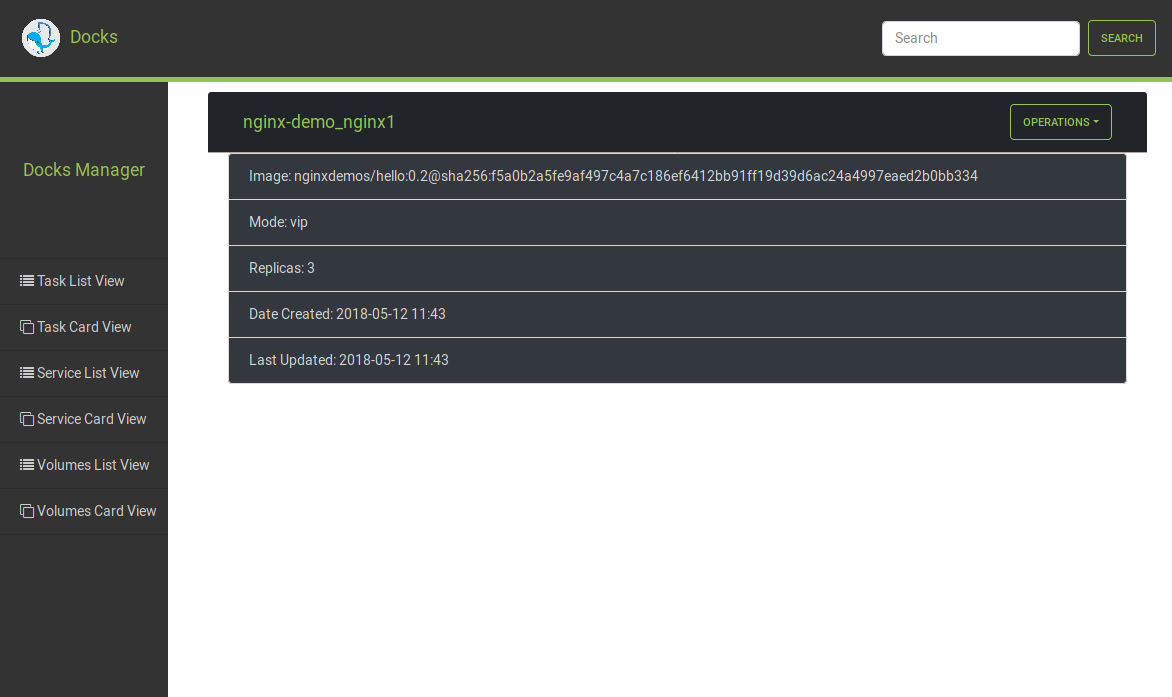
\includegraphics[scale=0.4]{service_list.png}
	\caption{Task list view, with one task expanded}
\end{figure}

The services card view will display the following information:
\begin{itemize}
	\tightlist
	\item Service name
	\item Image the service is created from
	\item The mode of the service. \texttt{vip} - Virtual IP, the service is assigned an IP address and will distribute the requests to the replicated tasks.
	\item The number of replicas of the service. Each replica represents a task in the swarm.
	\item Last updated
\end{itemize}

\begin{figure}[H]
	\centering
	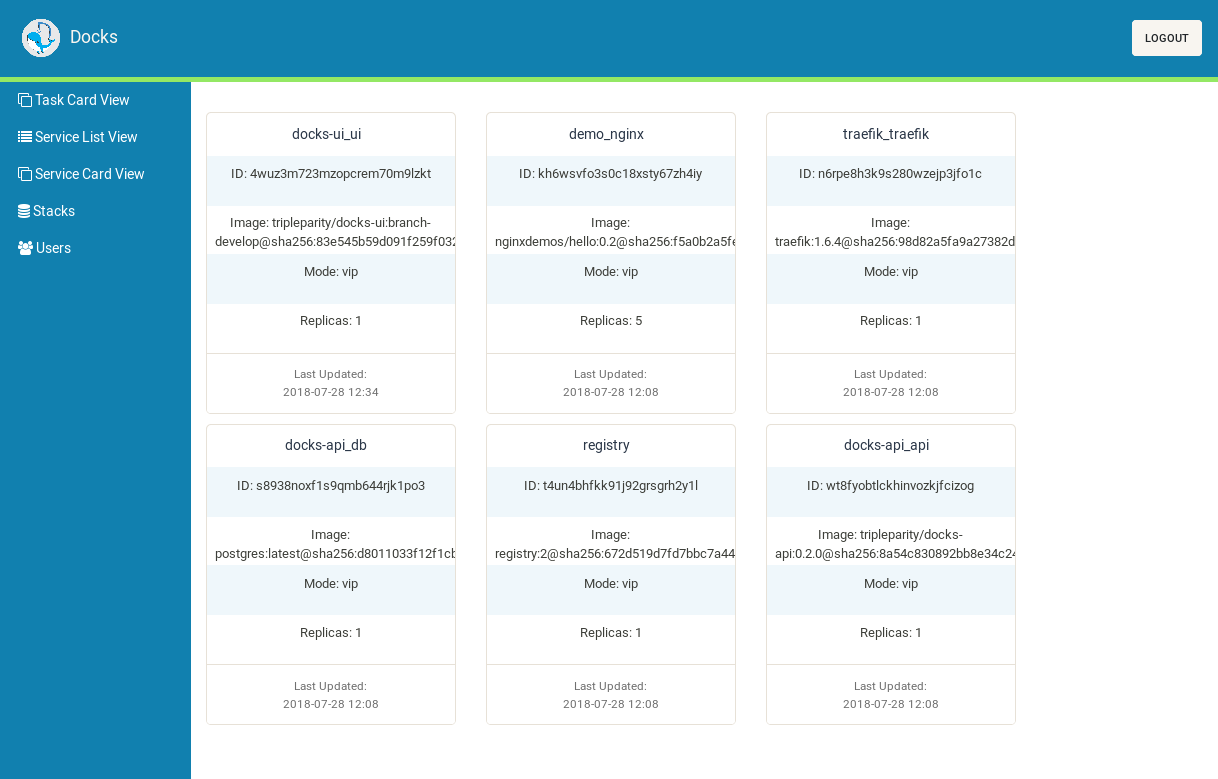
\includegraphics[scale=0.4]{service_card_view.png}
	\caption{Services card view}
\end{figure}

When clicking on a Service Card the following additional information will be displayed:
\begin{itemize}
	\tightlist
	\item Ports the services makes use of
	\item Tasks associated with the service
	\item Date Created
\end{itemize}

\begin{figure}[H]
	\centering
	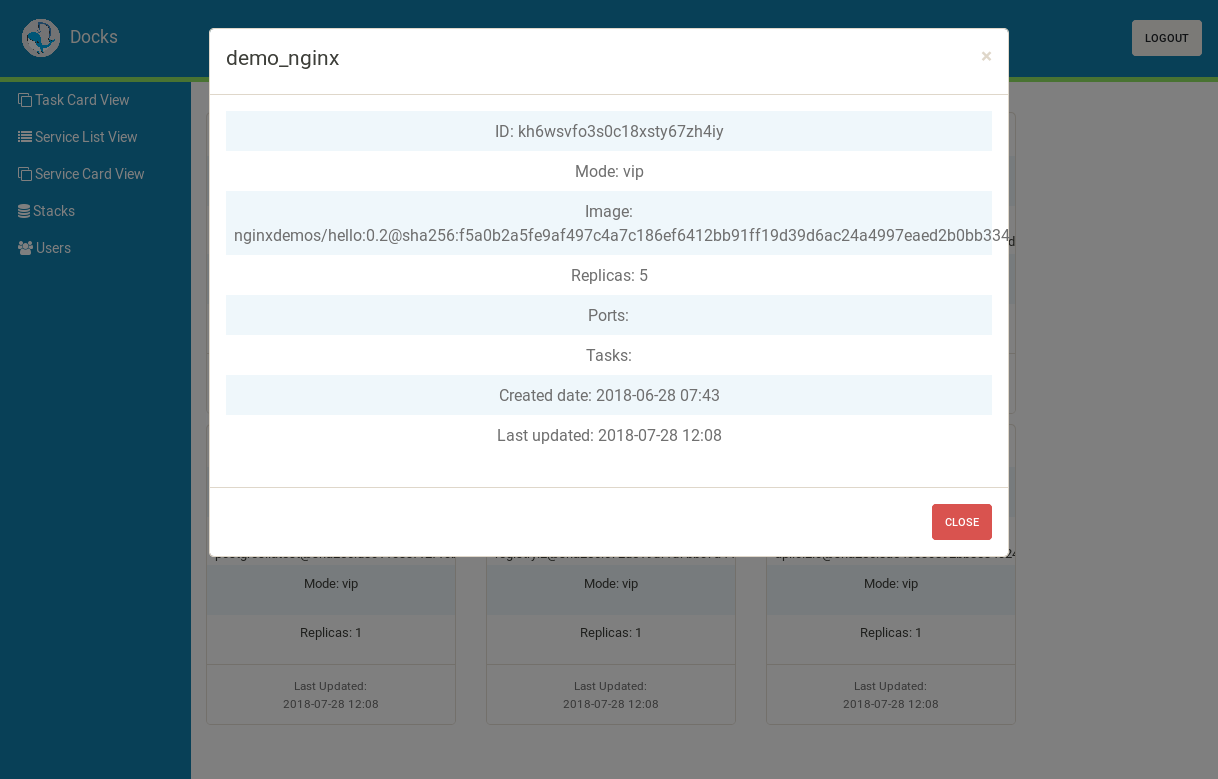
\includegraphics[scale=0.4]{service_card_modal.png}
	\caption{Services card view}
\end{figure}

\subsubsection{Service Operations}
From the list view you can perform the following operations by clicking on the \texttt{Operations} button:
\begin{itemize}
	\tightlist
	\item Scale the service
	\item Update the service
	\item View the service logs
	\item Remove the service from the swarm
\end{itemize}

\begin{figure}[H]
	\centering
	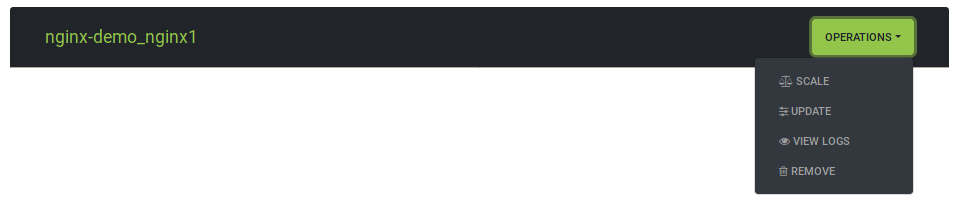
\includegraphics[scale=0.4]{service_list_operations.png}
	\caption{Service list operations}
\end{figure}

You can scale the service to change the number of replicas (tasks) of the service to run distribute on the swarm.
This is useful if the service needs more resources to handle more requests.

\begin{figure}[H]
	\centering
	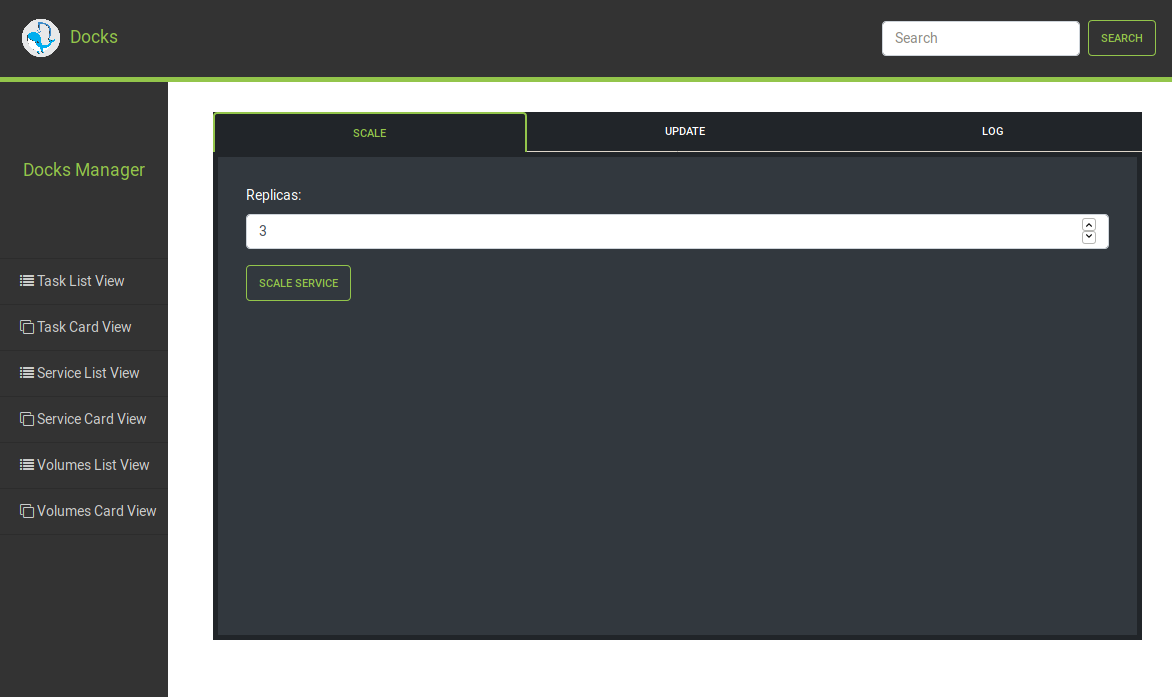
\includegraphics[scale=0.4]{service_list_scale.png}
	\caption{Service list operations}
\end{figure}

The service name and mode can be changed under the \texttt{Update} tab
\begin{figure}[H]
	\centering
	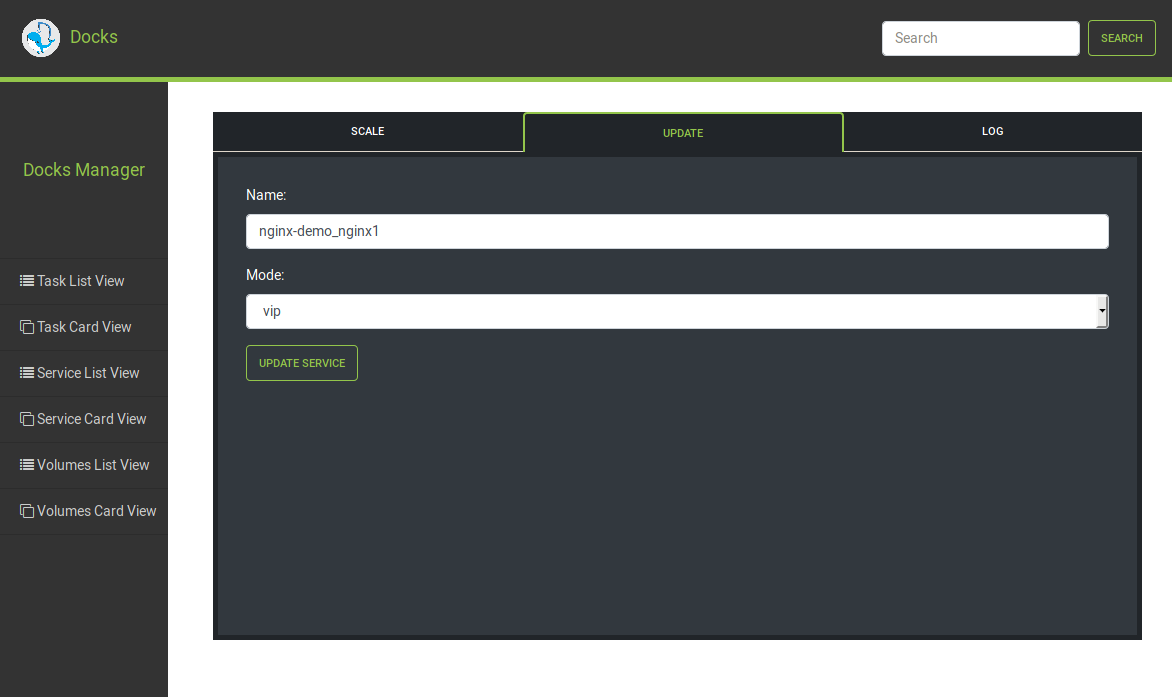
\includegraphics[scale=0.4]{service_list_update.png}
	\caption{Service list operations}
\end{figure}

The service log can be viewed under the \texttt{Log} tab. This is an aggregate log for all the tasks
associated with the service.
\begin{figure}[H]
	\centering
	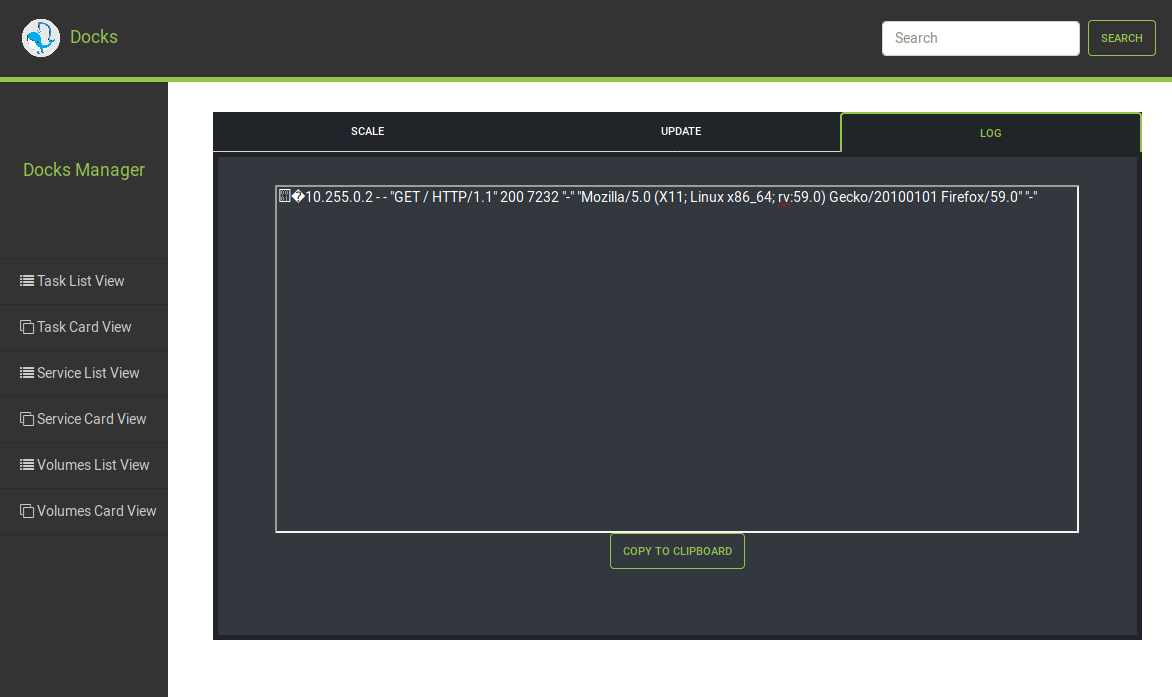
\includegraphics[scale=0.4]{service_list_log.png}
	\caption{Service list operations}
\end{figure}

\subsection{Volumes}

The volumes list view will display the following information when expanded:
\begin{itemize}
	\tightlist
	\item Driver the volume is using.
	\item Where the volume is mounted on the host
	\item Scope of the volume. Can be local or swarm wide
	\item Optional labels
	\item Further options
	\item Date created
\end{itemize}

\begin{figure}[H]
	\centering
	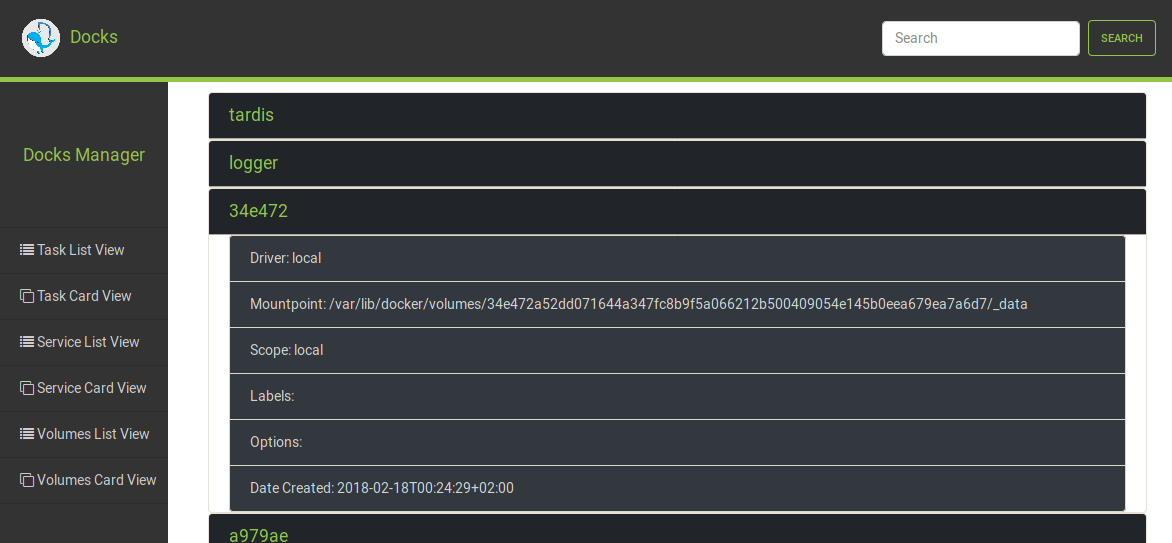
\includegraphics[scale=0.4]{volume_list.png}
	\caption{Volume list view, with an expanded item}
\end{figure}

The volumes card view will display the following information:
\begin{itemize}
	\tightlist
	\item Date created
	\item Driver the volume is using.
	\item Where the volume is mounted on the host
\end{itemize}

\begin{figure}[H]
	\centering
	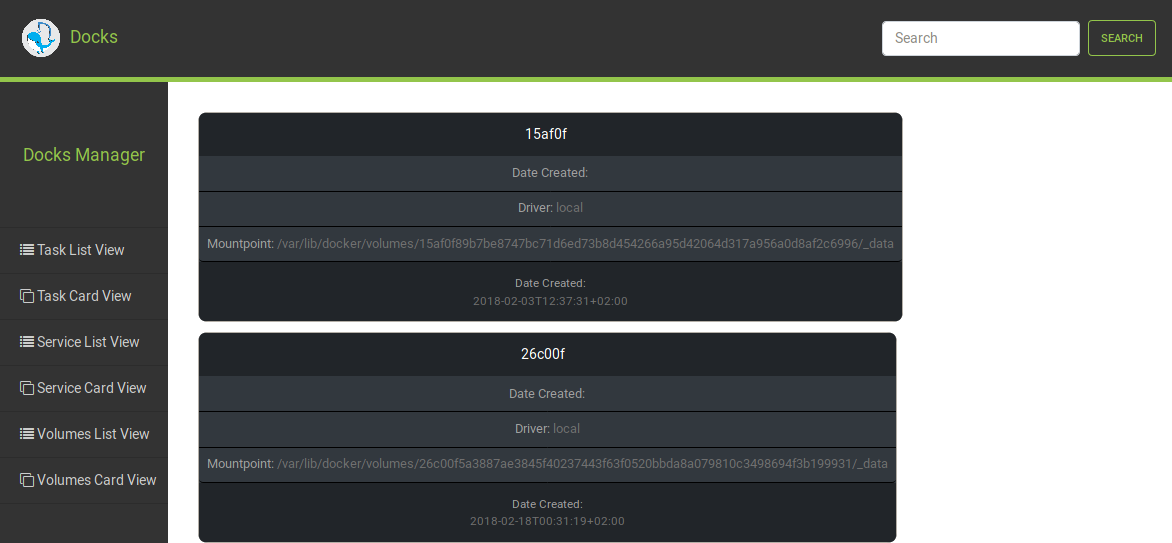
\includegraphics[scale=0.4]{volume_card_view.png}
	\caption{Volume list view, with an expanded item}
\end{figure}


\subsection{Updating Docks}
Docks can be updated by running \texttt{sudo docker-compose pull} and then
\texttt{docker-compose up --force-recreate} in the \texttt{docks} cloned repository


\section{Troubleshooting}
\subsection{Error: bind: address already in use}
Another service is most likely running on port \texttt{4200}, \texttt{8080} or \texttt{8081}.
The ports for Docks and nginx-demo can be specified in the \emph{docker-compose.yml} 
and \emph{docker-compose-yml} files.

For example to run on port 9000 instead of 4200 make the following changes:

\begin{lstlisting}
    ports:
      - 4200:80
\end{lstlisting}
to
\begin{lstlisting}
    ports:
      - 9000:80
\end{lstlisting}


\end{document}
